% English version. Compile with XeLaTeX or pdfLaTeX (Overleaf), or `tectonic -X compile main_en.tex`.
% Tables and numbers in generated/en/ are produced by make_tables.py from reports/evidence/.
\documentclass[sigconf,nonacm]{acmart}

\usepackage[english]{babel}
\usepackage{booktabs}
\usepackage{array}
\usepackage{amsmath}

% Auto-generated by make_tables.py - do not edit
\newcommand{\FZeroAP}{0.171}
\newcommand{\FZeroVal}{0.064}
\newcommand{\FZeroFone}{0.246}
\newcommand{\FZeroPk}{0.318}
\newcommand{\FZeroRk}{0.177}
\newcommand{\FZeroHits}{318}
\newcommand{\FOneAP}{0.534}
\newcommand{\FOneVal}{0.477}
\newcommand{\FOneFone}{0.534}
\newcommand{\FOnePk}{0.712}
\newcommand{\FOneRk}{0.396}
\newcommand{\FOneHits}{712}
\newcommand{\FTwoAP}{0.662}
\newcommand{\FTwoVal}{0.583}
\newcommand{\FTwoFone}{0.664}
\newcommand{\FTwoPk}{0.893}
\newcommand{\FTwoRk}{0.497}
\newcommand{\FTwoHits}{893}
\newcommand{\FThreeAP}{0.610}
\newcommand{\FThreeVal}{0.521}
\newcommand{\FThreeFone}{0.589}
\newcommand{\FThreePk}{0.798}
\newcommand{\FThreeRk}{0.444}
\newcommand{\FThreeHits}{798}
\newcommand{\FFourAP}{0.684}
\newcommand{\FFourVal}{0.592}
\newcommand{\FFourFone}{0.685}
\newcommand{\FFourPk}{0.915}
\newcommand{\FFourRk}{0.509}
\newcommand{\FFourHits}{915}
\newcommand{\FFourPkPct}{91.50}
\newcommand{\FFourRkPct}{50.89}
\newcommand{\FZeroAPpre}{0.071}
\newcommand{\FZeroAPpost}{0.973}
\newcommand{\FOneAPpre}{0.333}
\newcommand{\FOneAPpost}{0.962}
\newcommand{\FTwoAPpre}{0.506}
\newcommand{\FTwoAPpost}{0.958}
\newcommand{\FThreeAPpre}{0.413}
\newcommand{\FThreeAPpost}{0.962}
\newcommand{\FFourAPpre}{0.528}
\newcommand{\FFourAPpost}{0.961}
\newcommand{\EZeroAP}{0.670}
\newcommand{\EZeroFone}{0.673}
\newcommand{\ERAP}{0.662}
\newcommand{\ERFone}{0.664}
\newcommand{\ERDisc}{0.502}
\newcommand{\ERKS}{0.019}
\newcommand{\EOneAP}{0.673}
\newcommand{\EOneFone}{0.674}
\newcommand{\EOneDisc}{0.647}
\newcommand{\EOneKS}{0.047}
\newcommand{\ETwoAP}{0.648}
\newcommand{\ETwoFone}{0.625}
\newcommand{\ETwoDisc}{0.999}
\newcommand{\ETwoKS}{0.221}
\newcommand{\ELLMaAP}{0.609}
\newcommand{\ELLMaFone}{0.588}
\newcommand{\ELLMaDisc}{0.983}
\newcommand{\ELLMaKS}{0.126}
\newcommand{\ELLMbAP}{0.597}
\newcommand{\ELLMbFone}{0.493}
\newcommand{\ELLMbDisc}{0.996}
\newcommand{\ELLMbKS}{0.139}
\newcommand{\ERDelta}{$-$0.0077}
\newcommand{\EOneDelta}{0.0026}
\newcommand{\ETwoDelta}{$-$0.0221}
\newcommand{\ELLMaDelta}{$-$0.0611}
\newcommand{\ELLMbDelta}{$-$0.0732}


\settopmatter{printfolios=true}
\setlength{\emergencystretch}{1.5em}

\begin{document}

\title{Money Laundering Detection with Machine Learning}
\subtitle{Course project, Information Systems Security}

\author{Nguyễn Thế Vĩnh}
\email{26848266@grad.uit.edu.vn}
\affiliation{%
  \institution{University of Information Technology, VNU-HCM}
  \city{Ho Chi Minh City}
  \country{Vietnam}}

\author{Hoàng Đức Chung}
\email{26848014@grad.uit.edu.vn}
\affiliation{%
  \institution{University of Information Technology, VNU-HCM}
  \city{Ho Chi Minh City}
  \country{Vietnam}}

\author{Nguyễn Hải Đăng}
\email{26848027@grad.uit.edu.vn}
\affiliation{%
  \institution{University of Information Technology, VNU-HCM}
  \city{Ho Chi Minh City}
  \country{Vietnam}}

\renewcommand{\shortauthors}{Nguyễn Thế Vĩnh, Hoàng Đức Chung, and Nguyễn Hải Đăng}

\begin{abstract}
Machine learning for money laundering detection faces two obstacles: the positive class is extremely rare, and
the signal lies in behavioral context rather than in individual transactions. We compare two ways of improving a
detector within a single evaluation protocol on the 5,078,345 transactions of the synthetic IBM AML HI-Small
dataset: \emph{data augmentation} of the positive class with random oversampling, SMOTENC, CTGAN, and a Large
Language Model (LLM), and \emph{better representations} through temporal behavioral features. We build 63 features
describing account history, windowed activity, and counterparty relationships, computed strictly from transactions
that occur before the prediction time, and keep an XGBoost classifier fixed. Adding the feature groups step by step
raises Average Precision (AP) from \FZeroAP{} to \FOneAP{} and \FFourAP; with an alert budget of the 1,000
highest-scoring transactions, the full configuration reaches \FFourPkPct\% precision and \FFourRkPct\% recall. In
contrast, no augmentation method clearly improves over no augmentation; the two LLM variants lower AP from
\EZeroAP{} to \ELLMaAP{} and \ELLMbAP, and the samples generated by CTGAN or the LLM are almost perfectly separable
from real data (discriminator AUC $\geq$ \ELLMaDisc). A further analysis reveals a strong distribution shift starting
on September 11, 2022; on the part of the test set before that date, the benefit of behavioral features persists.
For transaction data, feature quality and the temporal correctness of the pipeline matter more than adding
synthetic data.
\end{abstract}

\keywords{anti-money laundering, transaction monitoring, XGBoost, temporal features, feature engineering,
data augmentation, large language models, data leakage}

\maketitle
\pagestyle{plain}  % no running head (title/authors) on later pages, page number only

% ======================================================================
\section{Introduction}

Money laundering disguises the illicit origin of funds through chains of transactions. Financial institutions must
monitor transactions and report suspicious activity under the FATF Recommendations~\cite{fatf2012} and, in Vietnam,
under the 2022 Law on Anti-Money Laundering~\cite{luatpcrt2022en}. From an information security perspective, a
transaction monitoring system plays a role similar to an intrusion detection system: it must rank a very large
stream of events of which only a small fraction is malicious, and every false positive costs investigator time.

Machine learning for money laundering detection faces three difficulties. First, the positive class is extremely
rare: in the IBM AML HI-Small dataset~\cite{altman2023realistic} only about 0.1\% of transactions are labeled as
laundering. Second, a single transaction carries almost no signal; the evidence lies in its \emph{context}, such as
account history, transaction velocity, and relationships between accounts. Third, the data is ordered in time, so it
is easy to let the model ``see the future'' during feature engineering (temporal leakage), which produces
over-optimistic results.

There are two common ways to improve a detector. The first is \emph{data augmentation} of the positive class through
oversampling, SMOTE~\cite{chawla2002smote}, generative models such as CTGAN~\cite{xu2019ctgan}, or, more recently,
LLMs~\cite{borisov2023great,seedat2024cllm}. The second is \emph{feature engineering} that describes the temporal
behavior of accounts and the relationships between them~\cite{blanusa2024gfp,deprez2024network}. We compare both
under one protocol: the same temporal split, the same XGBoost classifier~\cite{chen2016xgboost} with fixed
hyperparameters, the same threshold selection on the validation set, and three seeds. Our contributions are:

\begin{itemize}
  \item A set of 63 behavioral features computed \emph{strictly in time}: only transactions with an earlier timestamp
  are used, transactions within the same minute share one history snapshot, and money totals are kept separate per
  currency.
  \item A controlled ablation over five predefined configurations, showing that AP grows from \FZeroAP{} to
  \FFourAP{} and that every added group improves AP for all three seeds.
  \item An evaluation of four data augmentation methods, including two LLM-based generators, together with quality
  diagnostics of the synthetic data. None clearly improves the detector; CTGAN and LLM samples are almost perfectly
  separable from real data.
  \item An analysis of evaluation validity covering the time policy, a distribution shift starting on September 11,
  2022, and test-set reuse, together with a reproducible verification procedure.
\end{itemize}

% ======================================================================
\section{Related Work}

\paragraph{Datasets and benchmarks} Since real bank data cannot be published, academic work relies on public data
such as the Elliptic Bitcoin transaction graph~\cite{weber2019elliptic} or on simulated data. Altman et
al.~\cite{altman2023realistic} released the AMLworld agent-based generator and six fully labeled synthetic banking
datasets~\cite{ibmamlkaggle}; HI-Small is the smallest one with the higher illicit ratio.

\paragraph{Graph features and GNNs} The Graph Feature Preprocessor (GFP)~\cite{blanusa2024gfp}, part of Snap
ML~\cite{dunner2018snapml}, extracts fan-in/fan-out, scatter-gather, and cycle patterns together with windowed
vertex statistics in real time and feeds them to gradient boosting models; on HI-Small this reaches a
minority-class F1 of about 0.63--0.65 and outperforms standard Graph Neural Networks (GNNs).
Multi-GNN~\cite{egressy2024multignn} extends GNNs to directed multigraphs. Deprez et al.~\cite{deprez2024network}
survey 97 studies and find that network information improves predictive performance. Recent work focuses on fast
pattern mining~\cite{ye2026blazingaml} or quasi-temporal graph representations~\cite{tariq2026exstraqt}. In contrast,
Effendi and Chattopadhyay~\cite{effendi2024fhe} observe that XGBoost may not need graph features in some data
settings. We do not reproduce GFP; we focus on local behavioral and relationship statistics that are directly
interpretable.

\paragraph{Data augmentation and LLMs} SMOTE~\cite{chawla2002smote} interpolates between minority samples;
CTGAN~\cite{xu2019ctgan} learns tabular distributions with a conditional GAN. LLMs have been used to generate tabular
data~\cite{borisov2023great}, combined with data curation in low-data regimes~\cite{seedat2024cllm}, or to propose
features automatically~\cite{hollmann2023caafe,abhyankar2025llmfe}. We evaluate LLM-based generation of laundering
transactions in feature space for an extremely imbalanced problem.

% ======================================================================
\section{Data and Problem}

\paragraph{Dataset} We use the file \texttt{HI-Small\_Trans.csv} of IBM AML~\cite{ibmamlkaggle}, which contains
5,078,345 transactions between September 1 and 18, 2022, of which 5,177 (0.102\%) are labeled as laundering. Each
transaction has a timestamp (minute resolution), sender and receiver bank and account, amount and currency on both
sides, payment format, and label. The file is checked with a SHA-256 hash between the local and Kaggle environments.
Accounts are identified by the bank--account pair; identifiers are only used to look up history and are never model
inputs.

\paragraph{Task} Each transaction is a sample. The model outputs a suspicion score for ranking; binary decisions use
a threshold chosen on the validation set. Scores are not calibrated as risk probabilities.

\paragraph{Temporal split} Transactions are sorted by timestamp and split approximately 60/20/20; each cut is moved to
the start of its minute so that no minute is split across two sets (Table~\ref{tab:split}). The data is not shuffled,
and validation and test labels are never used for feature engineering or training.

\begin{table}[t]
\caption{Temporal split of the data.}
\label{tab:split}
\small
\setlength{\tabcolsep}{3pt}
\begin{tabular}{lrrrl}
\toprule
Set & Transactions & Positives & Rate & Time range \\
\midrule
Train & 3,046,861 & 2,297 & 0.075\% & Sep 1 -- Sep 6 13:35 \\
Validation & 1,015,602 & 1,082 & 0.107\% & Sep 6 13:36 -- Sep 8 16:11 \\
Test & 1,015,882 & 1,798 & 0.177\% & Sep 8 16:12 -- Sep 18 \\
\bottomrule
\end{tabular}
\end{table}

% ======================================================================
\section{Method}

\subsection{Time policy}

Let $t$ be the timestamp of the transaction to be scored. The history that may be observed is
\begin{equation}
H(t) = \{\, j : t_j < t \,\}.
\end{equation}
Because timestamps only have minute resolution and the true order within a minute is unknown, all transactions with
the same timestamp share one history snapshot; the history is updated only after the whole group has been queried.
Features therefore do not depend on the row order of the file. A self-transfer creates one outgoing and one incoming
event, and the outgoing event of a transaction never becomes history for its own receiving side. A time window of
length $W$ is defined as $[t-W, t)$. Unlabeled transactions that already occurred in the validation and test periods
may contribute history to later transactions, which corresponds to observing the transaction stream over time.

\subsection{Behavioral features}

The feature set has four groups and 63 columns in total:
\begin{itemize}
  \item \textbf{Transaction (11):} log amount paid and received, hour, weekday, payment format, both currencies,
  same bank, self-transfer, currency conversion, and round amount.
  \item \textbf{History (17):} for both sender and receiver: number of previous transactions, number of outgoing and
  incoming transfers, mean log amount sent and received, time since the previous transaction, and number of
  transactions on the same day in total and per direction; plus the number of previous transactions of the
  sender$\to$receiver pair.
  \item \textbf{Activity (20):} for 1-hour and 24-hour windows, the count and log total amount per direction for each
  account, and the deviation of the current log amount from the historical mean log amount in the same direction.
  Totals and deviations are kept separate per account \emph{and currency}; different currencies are never added
  without an exchange rate. Sliding sums use Neumaier compensated summation so that no residual error remains when
  amounts of very different magnitude leave the window.
  \item \textbf{Relationship (15):} number of distinct counterparties per direction and window, previous transactions
  of the reverse pair, age and recency of the sender$\to$receiver relationship, pair counts within each window, and
  the 24-hour counterparty share (transactions A$\to$B divided by A's outgoing transfers).
\end{itemize}
Without history, counts and totals are 0, while means and time gaps are left as NaN for XGBoost to handle. Five
configurations were fixed before running: F0 = Transaction; F1 = F0 + History; F2 = F1 + Activity; F3 = F1 +
Relationship; F4 = F1 + Activity + Relationship. The difference F1$-$F0 measures the effect of history; F2$-$F1 and
F3$-$F1 measure each group's benefit once history is present; F4$-$F2 and F4$-$F3 measure what the remaining group
adds. Features are computed with linear per-account scans accelerated by Numba.

\subsection{Data augmentation}

Augmentation only adds synthetic laundering transactions to the training set; validation and test always contain
real data. The number of synthetic samples is 0.5 times the number of positive training samples (1,148 per run). We
compare: \textbf{ER} random oversampling of positive samples; \textbf{E1} SMOTENC on standardized features, with
categorical features taken as the mode of the nearest neighbors; \textbf{E2} CTGAN trained for 300 epochs on positive
samples only; and \textbf{E3a/E3b} a commercial LLM accessed through the OpenAI API that generates laundering
transactions as JSON from real examples, column statistics, and logical constraints between columns, where E3b also
describes the AMLworld laundering typologies in the prompt. LLM outputs are validated, deduplicated, and filtered
for verbatim copies of real rows; API cost is capped by a budget ledger. Synthetic data quality is measured by the
mean per-column Kolmogorov--Smirnov (KS) statistic against real positive samples and by the AUC of an XGBoost
discriminator that separates real from synthetic rows (\emph{discriminator AUC}; 0.5 means indistinguishable).

The augmentation experiment was run before the feature study, on a 28-feature pipeline corresponding to F1 that
processed transactions within the same minute in the stable row order of the file. Because the protocol differs, we
only compare augmentation methods with each other, not their absolute scores with F0--F4.

\subsection{Model and evaluation}

All configurations use XGBoost with at most 1,000 trees, learning rate 0.05, max depth 8, subsample and
colsample\_bytree 0.8, minimum child weight 1, the \texttt{hist} tree method on GPU, and early stopping after 100
rounds on validation AUC-PR. There is no per-configuration hyperparameter tuning and no class resampling. The
F1-maximizing threshold is selected on the validation set of each run and applied unchanged to the test set.

The primary metric is Average Precision (AP), computed with scikit-learn. We also report F1 at the threshold and
Precision@1000/Recall@1000: the fraction of laundering transactions among the 1,000 highest-scoring test
transactions, and the fraction of all laundering test transactions that appear in that list. Accuracy is not used
because positives are very rare. Each configuration is run with three seeds (0, 1, 2); tables show the mean $\pm$
sample standard deviation (SD), and comparisons use paired differences per seed. This SD reflects training
variability on the same test set, not a confidence interval over new transaction populations.

\subsection{Verification and reproducibility}

The pipeline has 43 regression tests covering time and window boundaries, self-transfers, currencies, invariance to
reordering rows with the same timestamp, independence from labels and future data, and agreement with a direct
computation on small samples. After the runs, the 30 prediction files of the 15 runs are re-checked for labels,
ordering, AP, threshold metrics, and validation-based threshold selection. A manifest records the hashes of the data
and source code, library versions, column lists, and split information. Runs were executed in a private Kaggle
notebook with two Tesla T4 GPUs, NumPy 2.2.6, pandas 2.3.3, scikit-learn 1.7.2, XGBoost 3.1.1, and Numba 0.61.2.

% ======================================================================
\section{Results}

\subsection{Feature group ablation}

\begin{table*}[t]
\caption{Feature group ablation (mean $\pm$ SD over three seeds). AP is reported on the test and validation sets;
the other metrics are on the test set.}
\label{tab:features}
\begin{tabular}{lrccccc}
\toprule
Configuration & Features & AP (test) & AP (validation) & F1 & Precision@1000 & Recall@1000 \\
\midrule
F0 Transaction & 11 & 0.171 $\pm$ 0.002 & 0.064 $\pm$ 0.001 & 0.246 $\pm$ 0.016 & 0.318 $\pm$ 0.007 & 0.177 $\pm$ 0.004 \\
F1 +History & 28 & 0.534 $\pm$ 0.037 & 0.477 $\pm$ 0.026 & 0.534 $\pm$ 0.028 & 0.712 $\pm$ 0.033 & 0.396 $\pm$ 0.018 \\
F2 +Activity & 48 & 0.662 $\pm$ 0.020 & 0.583 $\pm$ 0.014 & 0.664 $\pm$ 0.016 & 0.893 $\pm$ 0.013 & 0.497 $\pm$ 0.007 \\
F3 +Relationship & 43 & 0.610 $\pm$ 0.014 & 0.521 $\pm$ 0.026 & 0.589 $\pm$ 0.026 & 0.798 $\pm$ 0.016 & 0.444 $\pm$ 0.009 \\
F4 Combined & 63 & \textbf{0.684 $\pm$ 0.025} & \textbf{0.592 $\pm$ 0.023} & \textbf{0.685 $\pm$ 0.026} & \textbf{0.915 $\pm$ 0.013} & \textbf{0.509 $\pm$ 0.007} \\
\bottomrule

\end{tabular}
\end{table*}

Table~\ref{tab:features} shows that transaction attributes alone (F0) yield an AP of \FZeroAP. Adding account history
(F1) gives the largest jump, to \FOneAP. Once history is present, the Activity group (F2, \FTwoAP) contributes more
than the Relationship group (F3, \FThreeAP), and combining both (F4) reaches the highest AP, \FFourAP. The ranking of
configurations is the same on validation and test. Table~\ref{tab:fsdelta} shows that every addition improves AP for
all three seeds, including F4 over F2: the Relationship group still adds information when the Activity group is
present. Three seeds only describe the consistency of these runs and are not sufficient to claim statistical
significance.

\begin{table}[t]
\caption{Paired AP differences on the test set (same seed).}
\label{tab:fsdelta}
\small
\begin{tabular}{lccc}
\toprule
Comparison & Mean $\Delta$AP & SD & Seeds improved \\
\midrule
F1 $-$ F0 & +0.3631 & 0.0371 & 3/3 \\
F2 $-$ F1 & +0.1278 & 0.0165 & 3/3 \\
F3 $-$ F1 & +0.0765 & 0.0233 & 3/3 \\
F4 $-$ F1 & +0.1502 & 0.0122 & 3/3 \\
F4 $-$ F2 & +0.0224 & 0.0043 & 3/3 \\
F4 $-$ F3 & +0.0737 & 0.0112 & 3/3 \\
\bottomrule

\end{tabular}
\end{table}

\begin{figure}[t]
\centering
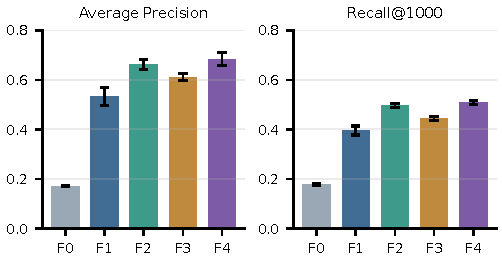
\includegraphics[width=\linewidth]{figures/feature_ablation.pdf}
\caption{AP and Recall@1000 of the five feature configurations; error bars show the SD over three seeds on the same
test set.}
\label{fig:ablation}
\end{figure}

\subsection{Alert budget}

The test set contains 1,798 laundering transactions. Among the 1,000 highest-scoring alerts, F1 finds about
\FOneHits{} laundering transactions on average and F4 finds \FFourHits; false positives drop accordingly while the
investigators' workload stays at 1,000 alerts. However, a recall of \FFourRk{} also means that almost half of the
laundering transactions fall outside the list. A budget of 1,000 alerts for the whole test set is an experimental
assumption; a real system may need daily limits or limits based on investigation capacity.

\subsection{Feature importance}

\begin{table}[t]
\caption{Ten features with the highest mean total-gain share in F4 (three seeds).}
\label{tab:importance}
\small
\begin{tabular}{r>{\raggedright\arraybackslash}p{4.1cm}lr}
\toprule
\# & Feature & Group & Gain (\%) \\
\midrule
1 & Sender's number of previous incoming transfers & History & 7.74 \\
2 & Receiver's time since its previous transaction & History & 7.05 \\
3 & Amount deviation from sender's outgoing history (same currency) & Activity & 6.35 \\
4 & Payment format & Transaction & 5.27 \\
5 & Hour of day & Transaction & 4.77 \\
6 & Previous transactions of the sender$\to$receiver pair & History & 4.64 \\
7 & Amount deviation from sender's incoming history & Activity & 4.29 \\
8 & Amount deviation from receiver's incoming history & Activity & 3.71 \\
9 & Log of amount received by sender in 24 hours & Activity & 3.70 \\
10 & Sender's mean log amount received & History & 3.51 \\
\bottomrule

\end{tabular}
\end{table}

Table~\ref{tab:importance} shows that the most important features combine the current transaction with account
context: the sender's number of previous incoming transfers, the receiver's time since its previous transaction, the
deviation of the amount from same-currency history, the payment format, and the number of previous transactions of
the account pair. This matches domain intuition: an account that has just received funds and forwards an amount that
is unusual for its history is a typical sign of a money mule. However, tree gain importance is affected by
correlations between columns, so it should not be read as a causal effect and does not replace the group ablation
above.

\subsection{Data augmentation}

\begin{table*}[t]
\caption{Training-set augmentation (earlier pipeline protocol, 28 features; three seeds). KS and discriminator AUC
measure the distance between synthetic and real positive samples; a discriminator AUC closer to 0.5 means more
realistic synthetic data.}
\label{tab:aug}
\begin{tabular}{lccccc}
\toprule
Method & AP & F1 & Precision@1000 & Mean KS & Discriminator AUC \\
\midrule
E0 No augmentation & 0.670 $\pm$ 0.008 & 0.673 $\pm$ 0.010 & 0.902 & -- & -- \\
ER Random oversampling & 0.662 $\pm$ 0.010 & 0.664 $\pm$ 0.003 & 0.894 & 0.019 & 0.502 \\
E1 SMOTENC & 0.673 $\pm$ 0.014 & 0.674 $\pm$ 0.009 & 0.899 & 0.047 & 0.647 \\
E2 CTGAN & 0.648 $\pm$ 0.014 & 0.625 $\pm$ 0.016 & 0.883 & 0.221 & 0.999 \\
E3a LLM, basic prompt & 0.609 $\pm$ 0.015 & 0.588 $\pm$ 0.018 & 0.854 & 0.126 & 0.983 \\
E3b LLM, AML-aware prompt & 0.597 $\pm$ 0.051 & 0.493 $\pm$ 0.181 & 0.838 & 0.139 & 0.996 \\
\bottomrule

\end{tabular}
\end{table*}

Table~\ref{tab:aug} shows that no augmentation method clearly improves over no augmentation (AP \EZeroAP). SMOTENC
reaches AP \EOneAP, a paired difference of only \EOneDelta{} that lies within the variation between seeds. Random
oversampling slightly lowers AP ($\Delta$AP = \ERDelta), CTGAN lowers it by \ETwoDelta, and the two LLM variants
lower it the most (\ELLMaDelta{} and \ELLMbDelta).

The discriminator AUC explains this pattern. Repeated samples are indistinguishable from real ones (\ERDisc), SMOTENC
reaches \EOneDisc, whereas CTGAN (\ETwoDisc) and the LLM (\ELLMaDisc{} and \ELLMbDisc) are almost perfectly
separable. Synthetic samples still carry a positive label, so the model learns regions that do not exist in real
data. With the LLM, precision at the threshold increases but recall drops sharply: the model becomes more
``conservative'' and misses more laundering transactions. Notably, adding domain knowledge about laundering
typologies to the prompt (E3b) does not help and makes results less stable across seeds (large F1 SD). In
transaction data, each laundering transaction is part of a chain with temporal and relational structure; generating
independent rows in feature space struggles to reproduce these constraints. This is the practical reason why we
shifted our focus to feature engineering.

\subsection{Temporal distribution shift}

Daily statistics show that from September 11, 2022 the transaction volume drops sharply while the positive rate
jumps (Figure~\ref{fig:daily}): September 10 has 208,325 transactions and 442 positives, whereas September 11 has
only 396 transactions but 232 positives. Within the test set, the part before September 11 contains 1,014,774
transactions with 1,143 positives (0.113\%), while the part from September 11 contains only 1,108 transactions but 655
positives (59.1\%). The cause has not been verified from the generation mechanism. Because this is a post-hoc
finding, we neither remove this part from the main evaluation nor retrain; instead, we split the fixed predictions
into two parts for diagnosis (Table~\ref{tab:temporal}).

\begin{table}[t]
\caption{AP on the two parts of the test set, split at September 11, 2022 (post-hoc diagnostic, same models).}
\label{tab:temporal}
\small
\begin{tabular}{lcc}
\toprule
Configuration & Before Sep 11 & From Sep 11 \\
\midrule
F0 & 0.071 $\pm$ 0.000 & 0.973 $\pm$ 0.000 \\
F1 & 0.333 $\pm$ 0.042 & 0.962 $\pm$ 0.004 \\
F2 & 0.506 $\pm$ 0.022 & 0.958 $\pm$ 0.005 \\
F3 & 0.413 $\pm$ 0.022 & 0.962 $\pm$ 0.004 \\
F4 & 0.528 $\pm$ 0.028 & 0.961 $\pm$ 0.005 \\
\bottomrule

\end{tabular}
\end{table}

\begin{figure}[t]
\centering
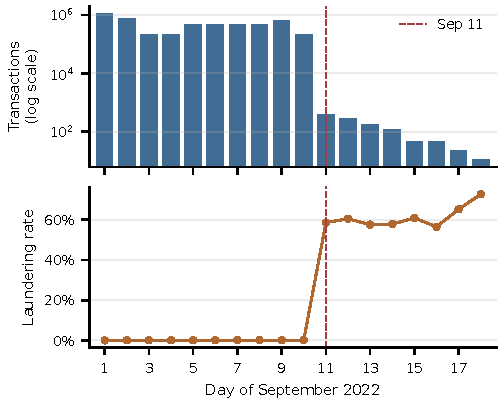
\includegraphics[width=\linewidth]{figures/daily_profile.pdf}
\caption{Daily transaction count (log scale) and positive rate in HI-Small; the dashed line marks September 11.}
\label{fig:daily}
\end{figure}

Before September 11, F4 still outperforms F1 (AP \FFourAPpre{} versus \FOneAPpre), so the benefit of the features does
not come only from the anomalous tail. In the tail, transaction attributes alone (F0) already reach AP \FZeroAPpost{}
and F4 does not outperform F0. Since AP depends on the positive rate, we only compare configurations within the same
part and do not compare AP across parts to conclude which part is easier.

\subsection{Computational cost}

On Kaggle, building the full feature table (including data loading and JIT compilation) takes about 35.0 seconds, and
the feature table occupies about 1.33 GB. Training the 15 models takes 620.2 seconds; the whole run, including
evaluation and file output, takes 733.3 seconds. These numbers describe one run in one environment; we have not
measured per-transaction feature update latency in an online service.

% ======================================================================
\section{Discussion}

\paragraph{Implications for information security} A transaction monitoring system is a defensive component; its
quality is measured by the number of laundering transactions found within the alert budget that investigators can
handle. Our results show that feature engineering determines effectiveness far more than adding synthetic data, and
behavioral features have the additional advantage of being explainable in business terms, which matters when alerts
must be reviewed by investigators. On the other hand, a behavior-based representation also creates an attack surface:
launderers can deliberately split transactions (structuring), spread them over time, or add money mules to distort
windowed and relational statistics (evasion attacks). In deployment, the system also needs access control for the
data and protection of API keys and alert results; our published code contains no API keys, raw data, or
per-transaction predictions.

\paragraph{Temporal leakage as a methodological vulnerability} A high score is meaningless if features use future
information, labels of the evaluation set, or an arbitrary row order of the file. The earlier augmentation pipeline
used 28 features corresponding to F1 but processed same-minute transactions in row order, and reached AP \EZeroAP{}
without augmentation, whereas F1 under the strict time policy reaches only \FOneAP. The two pipelines also differ in
some implementation details, so this is not a controlled comparison. Still, the large gap suggests that information
about same-minute transactions and their order in the file can inflate scores considerably. When comparing feature
sets or comparing with other work, the time policy must therefore be fixed and reported, just like the model and the
temporal split. For the same reason, the F1 of F4 (\FFourFone) should not be compared directly with published HI-Small
results~\cite{blanusa2024gfp,egressy2024multignn}: those works use different train/test cut points (for example,
Multi-GNN cuts at whole days), a fixed threshold instead of one chosen on validation, and different time handling.

\paragraph{Limitations} (i) The data is simulated; labels come from the generator, with no KYC, balances, or
verification of the source of funds. (ii) The HI-Small test set was examined in the earlier augmentation experiment,
so although the five configurations were predefined, the results remain exploratory. (iii) Three seeds only measure
training variability and do not establish statistical significance on independent data. (iv) Hyperparameters are
fixed, so the results show the effect of features under one training budget rather than maximum performance; some
runs reach or approach the 1,000-tree limit. (v) The mean log amounts in the History group still mix currencies.
(vi) The Relationship group only contains local statistics and does not detect cycles or multi-hop chains. (vii) The
augmentation experiment uses a different protocol. (viii) The tail of the test set has an anomalous distribution.
(ix) The results have not been validated on other AMLworld datasets or on real bank data.

% ======================================================================
\section{Conclusion}

On IBM AML HI-Small, behavioral feature engineering yields large and consistent gains, whereas synthetic data does
not. With a fixed XGBoost model, adding history, activity, and relationship features raises AP from \FZeroAP{} to
\FFourAP; among the 1,000 highest-scoring alerts, the full configuration reaches \FFourPkPct\% precision and
\FFourRkPct\% recall. The Activity group contributes more than the Relationship group when added alone, and the
Relationship group still helps when combined. Random oversampling, SMOTENC, CTGAN, and both LLM variants fail to
improve clearly; samples generated by CTGAN and the LLM are almost perfectly separable from real data. Results on the
test period before September 11 confirm the benefit of the features, while the anomalous tail is a reminder that
conclusions may not hold uniformly across all periods of the data.

Future work includes comparing with multi-hop graph pattern features such as GFP under the same time policy,
analyzing results per laundering typology, evaluating robustness against evasion strategies such as structuring or
money mules, and validating on other AMLworld datasets with a completely new held-out test set.

\paragraph{Reproducibility} Source code, configurations, tests, and per-run results are available at
\url{https://github.com/Chung10102004/atbmtt}. Raw data and per-transaction predictions are not included in the
repository.

\bibliographystyle{ACM-Reference-Format}
\bibliography{references}

\end{document}
